\documentclass{article}
\usepackage{graphicx}
\usepackage[section]{placeins}
\usepackage[a4paper,margin=0.75in]{geometry}
\usepackage{array}
\usepackage{varwidth}
\usepackage{tabularx}
\usepackage{amsmath}
\usepackage{subcaption}

\graphicspath{{../plots/}{images/}}

\title{COL380 Assignment 1 report \\  LU Decomposition using Pthreads and OpenMP}
\author{}
\date{}

\begin{document}

\maketitle

\section{Code overview}

Main Function:

\begin{enumerate}
    \item \textbf{Memory Allocation and Initialization}:
    \begin{itemize}
        \item Memory is dynamically allocated for the matrix \texttt{A}, matrices \texttt{L} and \texttt{U} (for LU decomposition), and an array \texttt{A\_old} to store a copy of the original matrix \texttt{A} for the purpose of calculating residual norm.
        \item A permutation vector \texttt{pi} is also allocated to keep track of row permutations during LU decomposition.
		\item \textbf{Pthreads}
		\begin{itemize}
			\item Here, each thread stores the required parameters, namely the pointers to the Matrices A, L, U and other paramters like starting row, ending row etc in a data structure called ThreadData. This is used for each thread separately.
		\end{itemize}
		\item \textbf{OpenMP}
		\begin{itemize}
			\item Here, we do not require the use of the thread data structure, it's implicitly handled by OpenMP.
		\end{itemize}
    \end{itemize}

    \item \textbf{Matrix Initialization for LU Decomposition}:
    \begin{itemize}
        \item Matrices \texttt{L} and \texttt{U} are initialized based on the requirements of LU decomposition.
        \item \texttt{L} is set to have 1s on the diagonal and zeros elsewhere below the diagonal.
        \item \texttt{U} is set to have elements of \texttt{A} on the diagonal and zeros elsewhere above the diagonal.
    \end{itemize}

    \item \textbf{LU Decomposition with Parallelization}:
    \begin{itemize}
        \item The LU decomposition algorithm is executed within a loop iterating over the columns of the matrix.
        \item Partial pivoting is performed within this loop, which involves finding the maximum element in the current column and swapping rows accordingly.
		\item \textbf{Pthreads}
		\begin{itemize}
			\item The work is divided into chunks to distribute evenly among threads. The number of rows each thread handles depends on the total number of threads and the current iteration of the outer loop.
			\item Pthreads are created and joined within the same loop to utilize parallelism effectively.
		\end{itemize}

		\item \textbf{OpenMP}
		\begin{itemize}
			\item For OpenMP, instead of explicitly dividing the work in chucks and distributing it evenly among threads, the OpenMP directive directly does the parallelization.
		\end{itemize}
    \end{itemize}

    \item \textbf{Memory Deallocation}:
    \begin{itemize}
        \item After the LU decomposition process is completed, memory allocated for matrices \texttt{A}, \texttt{L}, \texttt{U}, \texttt{A\_old}, and the permutation vector \texttt{pi} is deallocated using the \texttt{freeMemory} function.
    \end{itemize}

\end{enumerate}

Overall, while both versions achieve parallelization, the OpenMP version simplifies the process by providing a high-level interface for parallelism, whereas the Pthreads version requires more manual management of threads and data structures.

\clearpage

\section{Design decisions}

\begin{itemize}
	\item The specific part of the algorithm that is parallelized in this code is the update of the matrix A in the \verb|lu_decomposition| function. This operation involves subtracting the product of elements in the L and U matrices from the corresponding element in the A matrix.
	\item This operation is independent for each element of the matrix, meaning that the operation for one element does not depend on the result of the operation for any other element. This makes it a perfect candidate for parallelization, as it can be split up into smaller tasks that can be performed simultaneously by different threads.
	\item Hence we decided to parallelize that section, also considering the fact that it is the main bottleneck during processing.
\end{itemize}

\begin{figure}[!htb]
    \centering
    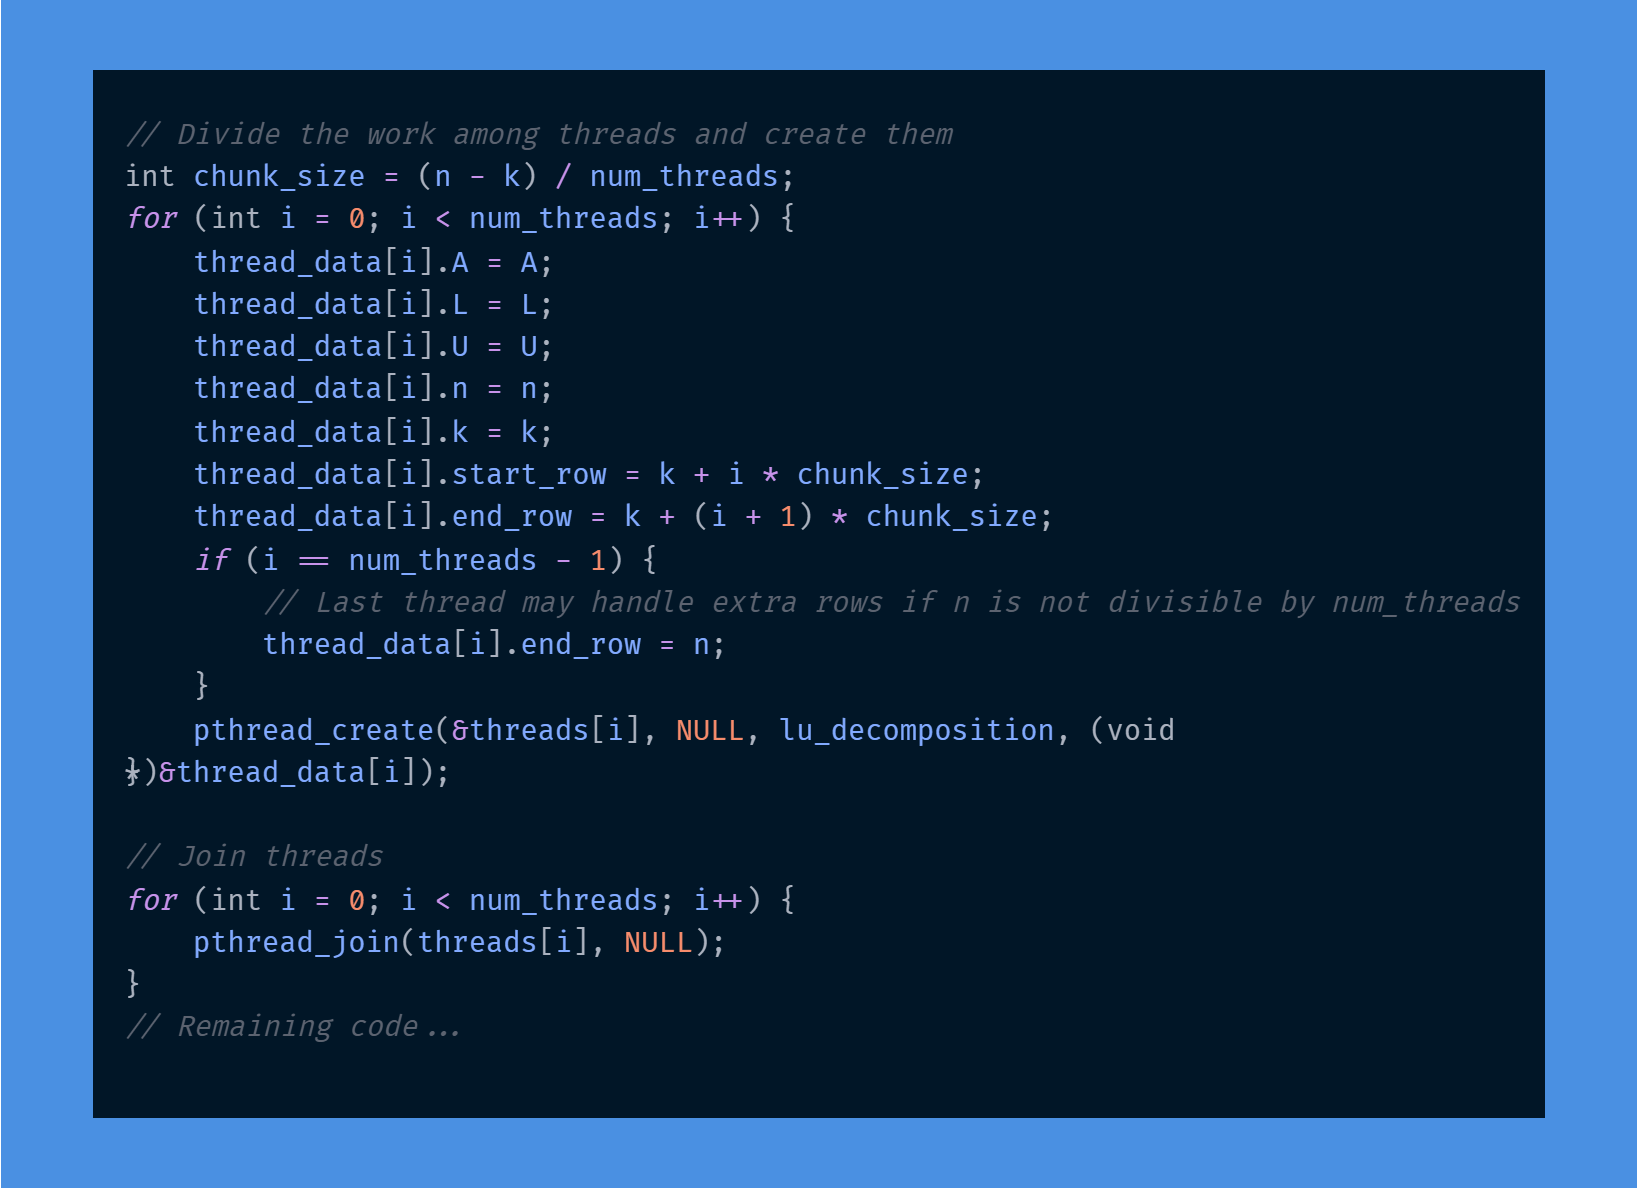
\includegraphics[width=13cm]{pthread_code.png}
    \caption{Parallelized code section for Pthreads}
    % \label{fig:1}
\end{figure}

\begin{figure}[!htb]
    \centering
    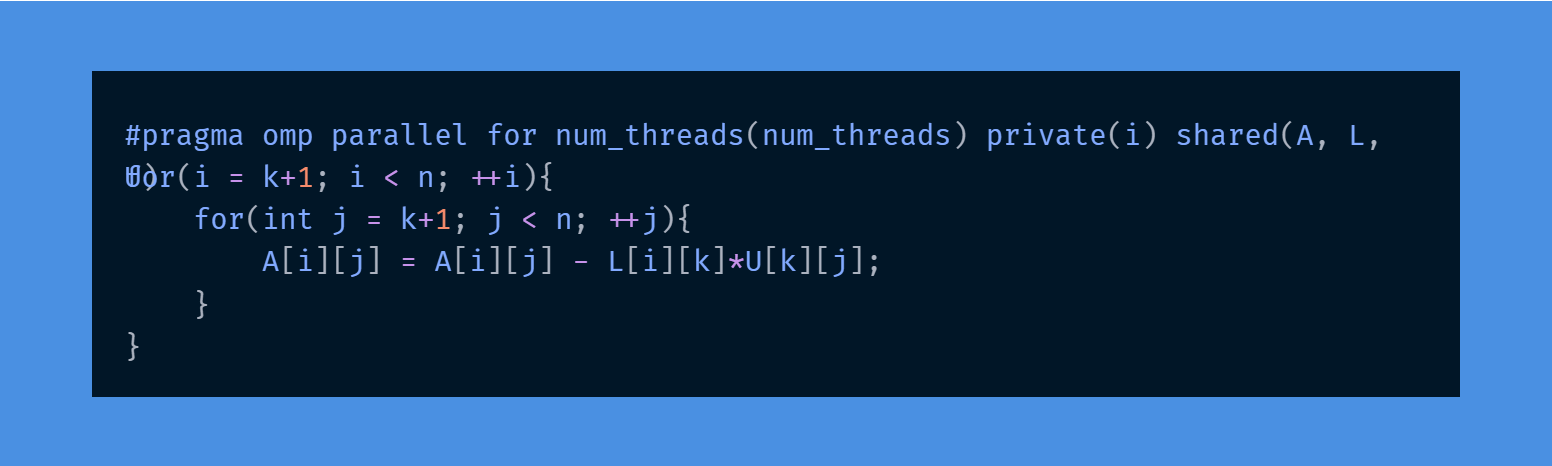
\includegraphics[width=13cm]{omp_code.png}
    \caption{Parallelized code section for OpenMP}
    % \label{fig:1}
\end{figure}

\clearpage

\section{Runtime Analysis}


\begin{table}[!htb]
	\centering
	\begin{tabular}{cccccc}
		\hline
		\multicolumn{1}{|c|}{n} & \multicolumn{1}{c|}{1 thread} & \multicolumn{1}{c|}{2 threads} & \multicolumn{1}{c|}{4 threads} & \multicolumn{1}{c|}{8 threads} & \multicolumn{1}{c|}{16 Threads} \\ \hline
		2000                    & 10.259                        & 5.223                          & 2.800                          & 2.389                          & 2.358                           \\
		4000                    & 80.641                        & 40.625                         & 23.366                         & 20.432                         & 20.939                          \\
		8000                    & 695.172                       & 350.163                        & 227.030                        & 181.928                        & 185.707                        
	\end{tabular}
	\caption{Time taken (in seconds) with Pthreads implementation}
	\label{pthreads_time_taken}
\end{table}

\begin{table}[!htb]
	\centering
	\begin{tabular}{cccccc}
		\hline
		\multicolumn{1}{|c|}{n} & \multicolumn{1}{c|}{1 thread} & \multicolumn{1}{c|}{2 threads} & \multicolumn{1}{c|}{4 threads} & \multicolumn{1}{c|}{8 threads} & \multicolumn{1}{c|}{16 Threads} \\ \hline
		2000                    & 7.533                         & 3.914                          & 2.147                          & 1.932                          & 1.943                           \\
		4000                    & 60.130                        & 34.073                         & 20.221                         & 17.029                         & 17.650                          \\
		8000                    & 478.16                        & 284.192                        & 183.303                        & 145.766                        & 153.070                        
	\end{tabular}
	\caption{Time taken (in seconds) with OpenMP implementation}
	\label{omp_time_taken}
\end{table}

Following are the obtained plots for Parallel efficiency vs number of threads:

% \begin{figure}[!htb]
%     \centering
%     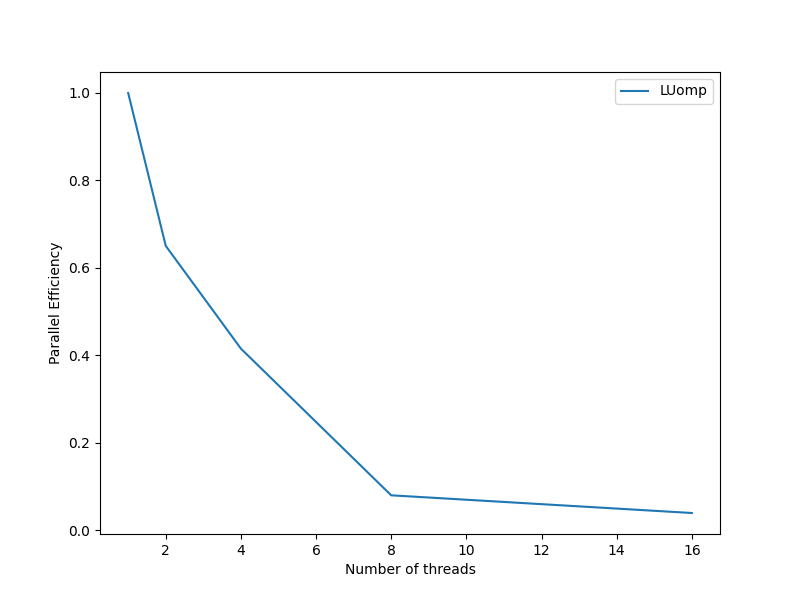
\includegraphics[width=13cm]{LUomp.png}
%     \caption{OpenMP}
%     % \label{fig:1}
% \end{figure}
%
% \begin{figure}[!htb]
%     \centering
%     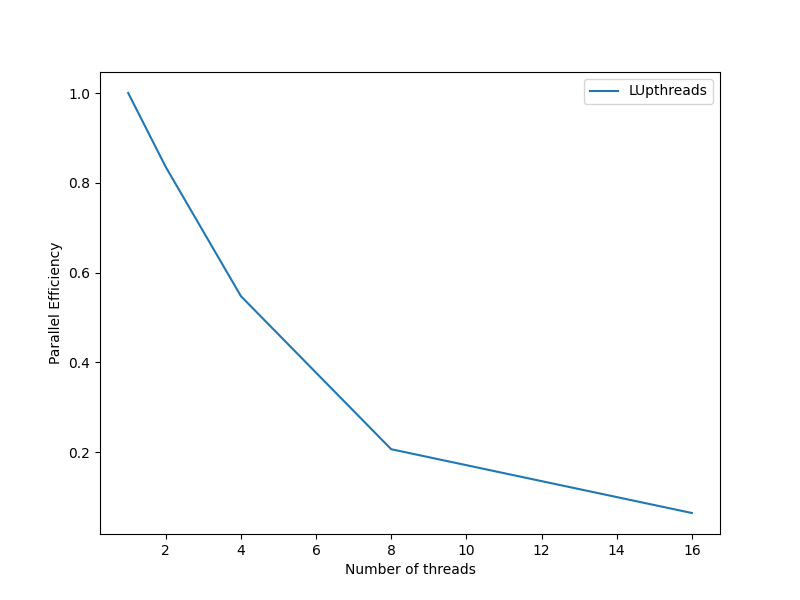
\includegraphics[width=13cm]{LUpthreads.png}
%     \caption{Pthreads}
%     % \label{fig:1}
% \end{figure}

\begin{figure}[!htb]
    \centering
    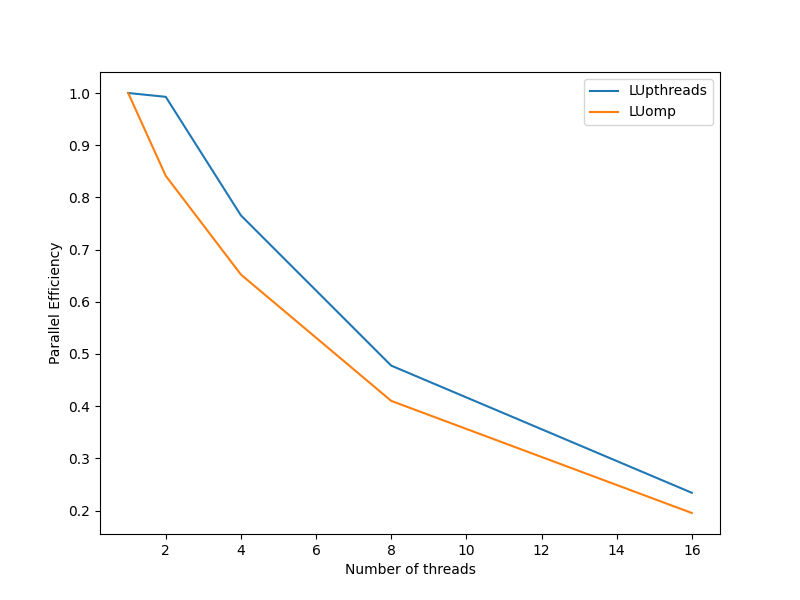
\includegraphics[width=15cm]{n8000/Both.png}
    \caption{For matrix of size $8000 \times 8000$ }
    % \label{fig:1}
\end{figure}

\clearpage

\section{Team info}

\subsection{Members}

\begin{table}[!htb]
	\centering
	\begin{tabular}{lll}
		  & Name                  & Entry Number \\
		1 & Sarthak               & 2020CS10379  \\
		2 & Brian Sajeev Katikkat & 2021CS50609  \\
		3 & Aman Hassan           & 2021CS50607 
	\end{tabular}
	\caption{}
	\label{team_members}
\end{table}

\subsection{Device specifications}

\begin{figure}[!htb]
    \centering
    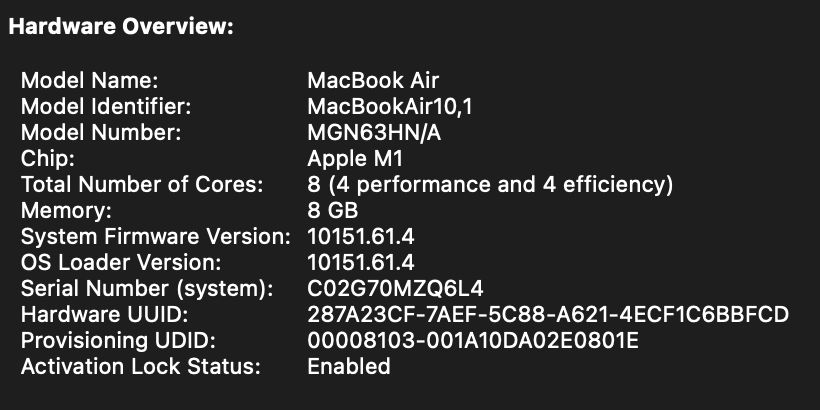
\includegraphics[width=13cm]{device_spec.jpg}
    \caption{Device specifications}
    % \label{fig:1}
\end{figure}

\end{document}
